% ==================================================
% 1. USE-CASE MODEL: SYSTEM OVERVIEW
% ==================================================
% Source of truth: the agreed UC-01 ... UC-20 specifications.
% Copy UC-Overview.png into sections/images/ before compiling.
% Required packages in main.tex: graphicx, caption, pdflscape, longtable.
%
% Each detailed UC diagram is already included in 02-use-case-specifications.tex.
% The optional 20-page gallery at the end of this file is OFF by default.
%
\clearpage
\section{Use-case Model}
\label{sec:use-case-model}

This section presents the overall use-case model of the Medication Safety
Assistant research prototype. It includes twenty use cases and five user
roles: Patient / General User, Healthcare Professional (HCP), Administrator,
Dataset Reviewer, and Technical Support. HCP review is simulated.
UC-19 is a future feature and is not included in the current implementation
scope.

\subsection{Use-Case Overview}
\label{subsec:uc-overview-table}

The following table uses the same IDs, names, and actors as the approved
use-case specifications. The overview diagram shows the main associations;
the detailed specifications describe Basic Flows, Alternative Flows,
preconditions, and postconditions.

\begingroup
\small
\setlength{\tabcolsep}{4pt}
\renewcommand{\arraystretch}{1.18}
\begin{longtable}{|p{0.11\textwidth}|p{0.51\textwidth}|p{0.30\textwidth}|}
\hline
\textbf{ID} & \textbf{Use-case Name} & \textbf{Actor(s)} \\ \hline
\endfirsthead
\hline
\textbf{ID} & \textbf{Use-case Name} & \textbf{Actor(s)} \\ \hline
\endhead
UC-01 & Sign In & All registered roles \\ \hline
UC-02 & Enter and Confirm Medication Information & Patient / General User \\ \hline
UC-03 & Check Medication Safety & Patient / General User \\ \hline
UC-04 & Arrange HCP Review & Patient / General User \\ \hline
UC-05 & Review Medication Safety Case & HCP; Patient / General User \\ \hline
UC-06 & Set Up Medication Reminders & Patient / General User \\ \hline
UC-07 & Manage Medication Reminders & Patient / General User \\ \hline
UC-08 & Record Dose Status & Patient / General User \\ \hline
UC-09 & View Adherence History & Patient / General User \\ \hline
UC-10 & View Medication and Safety History & Patient / General User \\ \hline
UC-11 & Ask a Medication Question & Patient / General User \\ \hline
UC-12 & Generate Patient Health Summary & Patient / General User \\ \hline
UC-13 & Share Patient Health Summary with HCP & Patient / General User \\ \hline
UC-14 & Review Medication Reference Data & Dataset Reviewer \\ \hline
UC-15 & Manage User Accounts and Roles & Administrator \\ \hline
UC-16 & Report Technical Issue & All registered roles \\ \hline
UC-17 & Handle Technical Support Request & Technical Support \\ \hline
UC-18 & Manage Patient Health Profile & Patient / General User \\ \hline
UC-19 & \emph{Manage Personal Medication Cabinet (Future Feature)} & Patient / General User \\ \hline
UC-20 & Manage Personal Account & All registered roles \\ \hline
\end{longtable}
\endgroup

% ==================================================
% OVERALL DIAGRAM -- A4 PORTRAIT, ENLARGED
% ==================================================
% On A4 portrait, normal text width is about 16 cm.  This image uses
% almost the full 21 cm page width (about 25% larger) while keeping
% the page, header, footer, and caption upright.
% Keep the length definition for the optional detailed gallery below.
\newlength{\UCModelPortraitWidth}
\setlength{\UCModelPortraitWidth}{\textwidth}

\clearpage
\subsection{Overall Use-Case Diagram}
\label{subsec:overall-use-case-diagram}
\begin{figure}[H]
  \centering
  \makebox[\textwidth][c]{%
    \IfFileExists{sections/images/UC-Overview.png}{%
      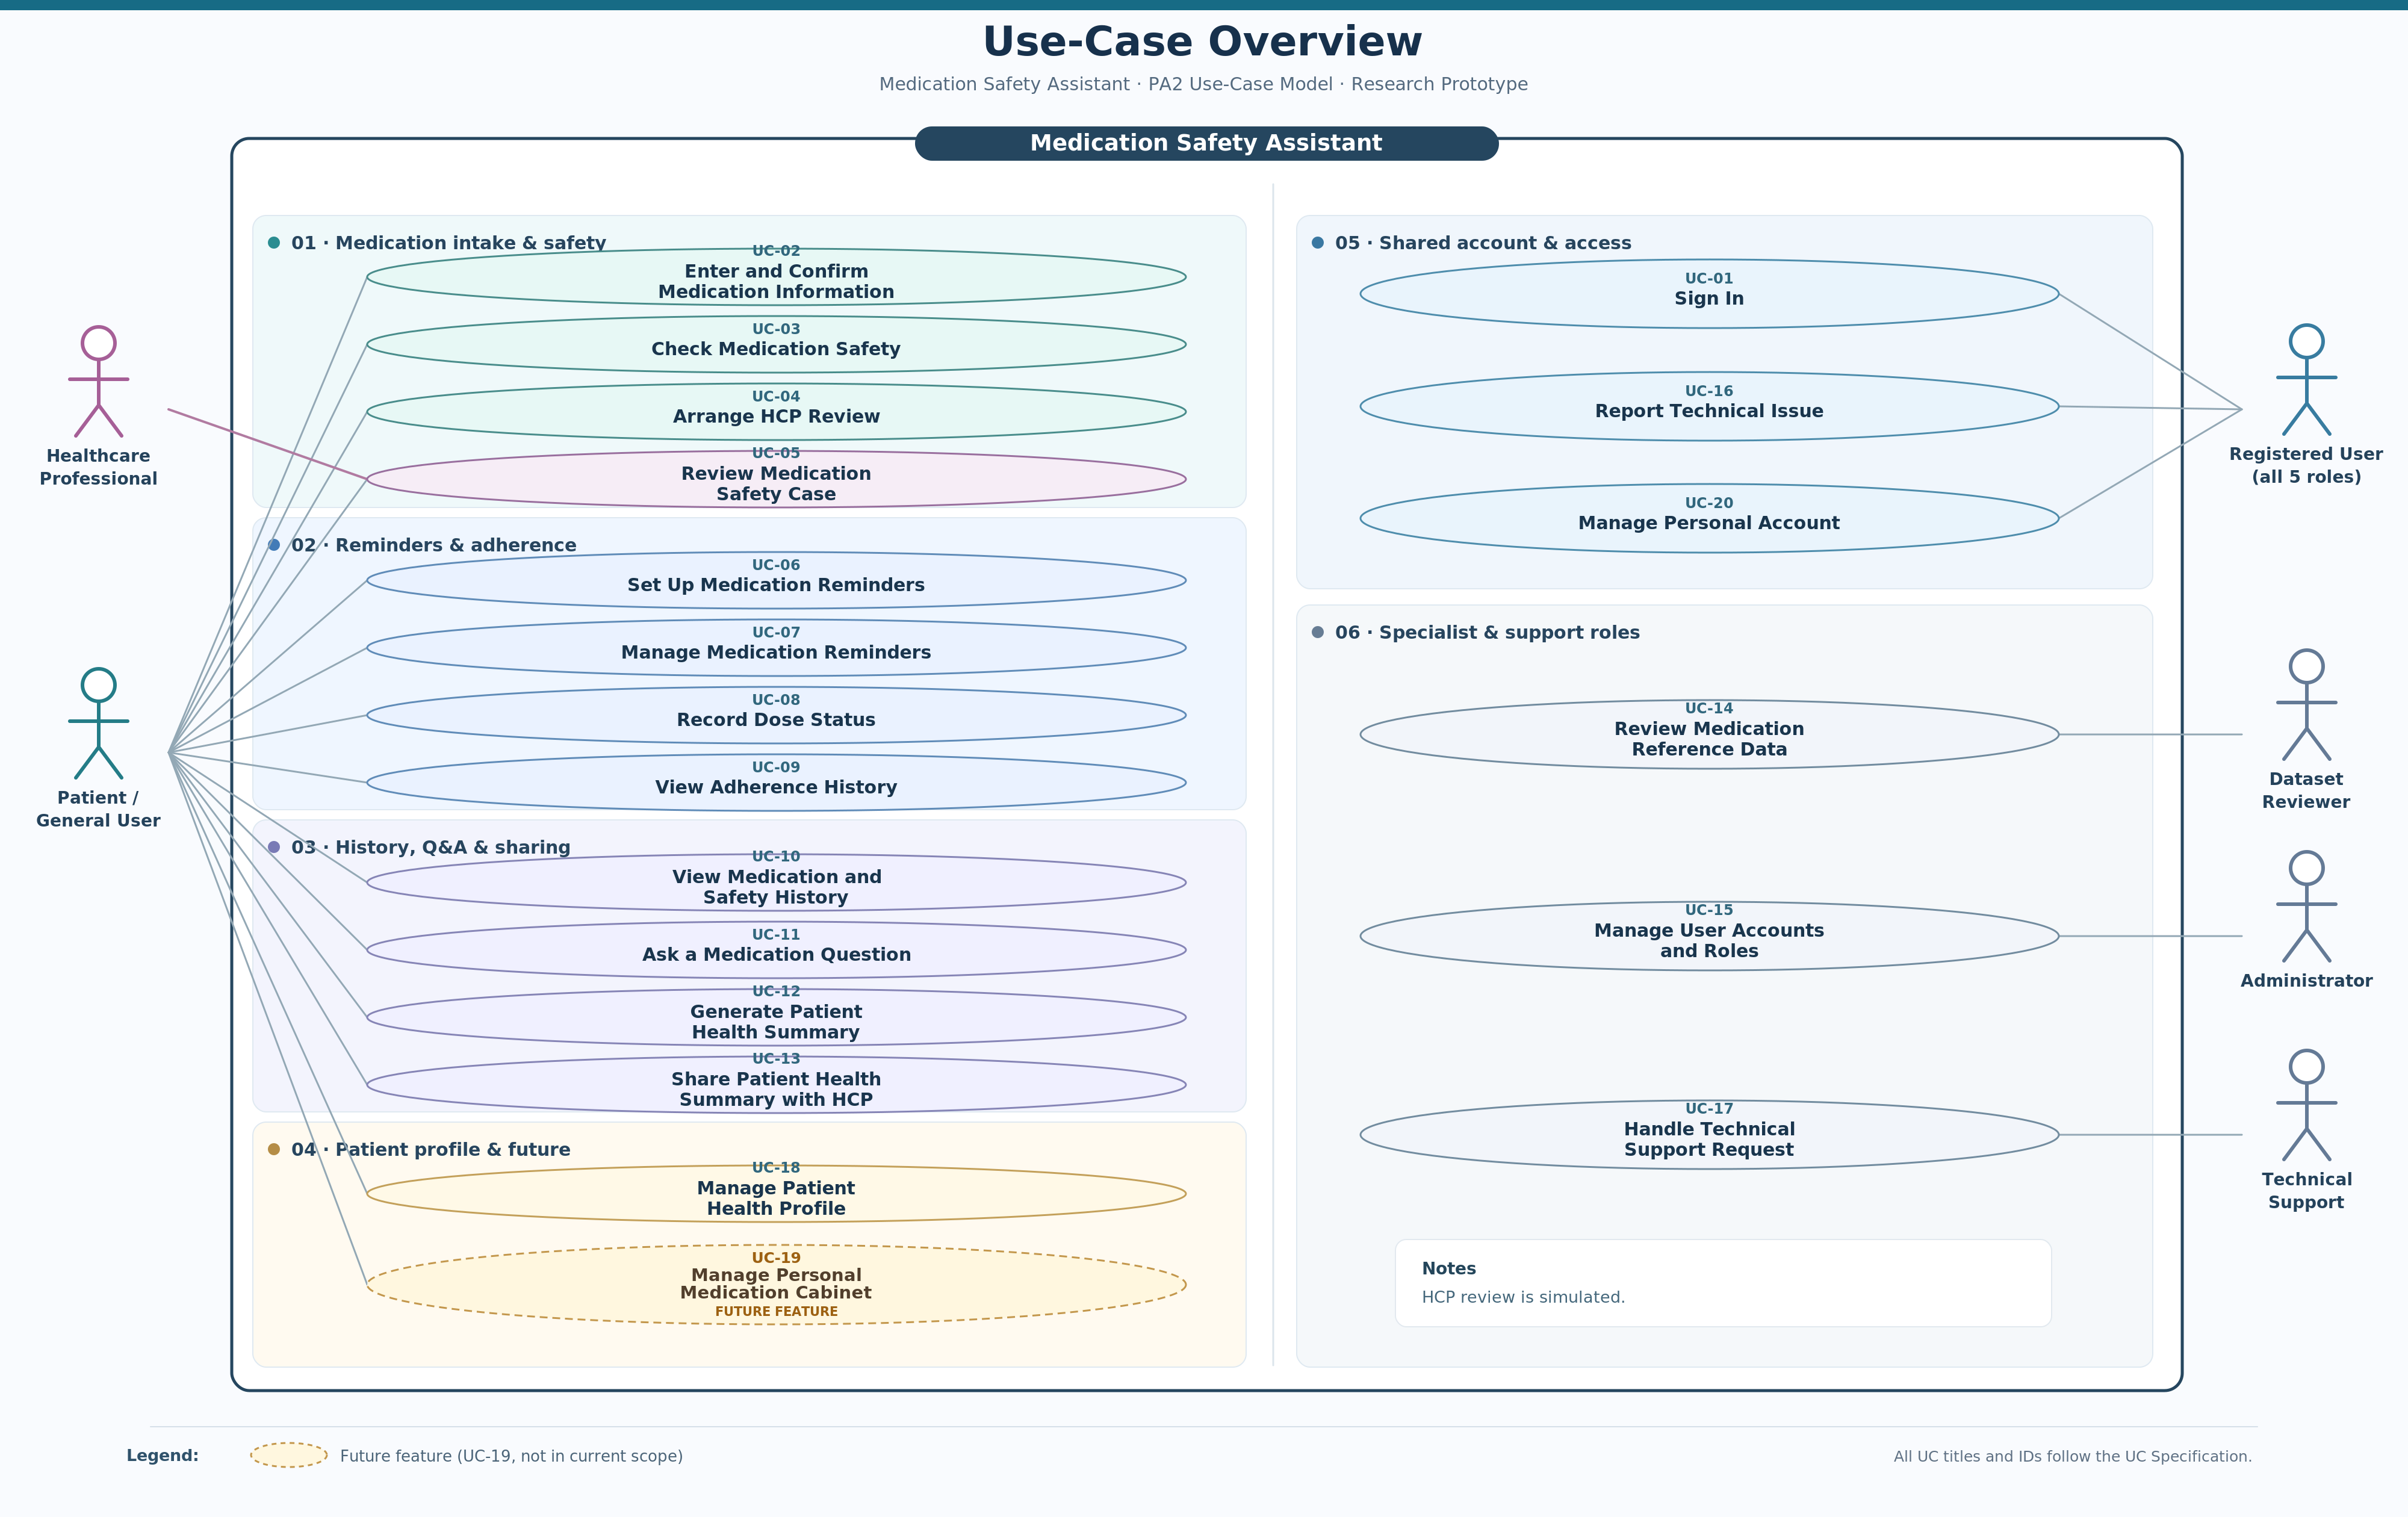
\includegraphics[
        width=\dimexpr\paperwidth-1cm\relax,
        height=0.78\textheight,
        keepaspectratio
      ]{sections/images/UC-Overview.png}%
    }{%
      \fbox{\parbox{0.90\textwidth}{\centering
        Missing image: \texttt{sections/images/UC-Overview.png}}}%
    }%
  }
  \caption{Medication Safety Assistant -- overall use-case diagram.}
  \label{fig:uc-overview}
\end{figure}

\clearpage
% ==================================================
% OPTIONAL FULL-PAGE DETAILED DIAGRAM GALLERY
% ==================================================
% Keep this OFF when 02-use-case-specifications.tex already contains
% the 20 diagrams. To produce a separate 20-page gallery instead, change
% \UCSeparateGalleryfalse to \UCSeparateGallerytrue AND remove the diagram
% insertions in section 02 to avoid duplicate figures.
\newif\ifUCSeparateGallery
\UCSeparateGalleryfalse

\ifUCSeparateGallery
  \subsection{Detailed Use-Case Diagrams}
  \newcommand{\UCModelImage}[1]{%
    \IfFileExists{sections/images/#1.pdf}{%
      \includegraphics[width=0.96\linewidth,height=0.76\UCModelPortraitWidth,keepaspectratio]{sections/images/#1.pdf}%
    }{%
      \IfFileExists{sections/images/#1.png}{%
        \includegraphics[width=0.96\linewidth,height=0.76\UCModelPortraitWidth,keepaspectratio]{sections/images/#1.png}%
      }{%
        \fbox{\parbox[c][0.25\UCModelPortraitWidth][c]{0.9\linewidth}{\centering Missing diagram: #1}}%
      }%
    }%
  }
  \newcommand{\UCModelFigure}[3]{%
    \clearpage
    \begin{landscape}
      \subsection{UC-#1: #2}
      \label{subsec:uc-model-#1}
      \begin{center}
        \UCModelImage{#3}%
        \captionof{figure}{UC-#1: #2 -- detailed use-case model.}
        \label{fig:uc-model-#1}
      \end{center}
    \end{landscape}
  }
  \UCModelFigure{01}{Sign In}{UC-01}
  \UCModelFigure{02}{Enter and Confirm Medication Information}{UC-02}
  \UCModelFigure{03}{Check Medication Safety}{UC-03}
  \UCModelFigure{04}{Arrange HCP Review}{UC-04}
  \UCModelFigure{05}{Review Medication Safety Case}{UC-05}
  \UCModelFigure{06}{Set Up Medication Reminders}{UC-06}
  \UCModelFigure{07}{Manage Medication Reminders}{UC-07}
  \UCModelFigure{08}{Record Dose Status}{UC-08}
  \UCModelFigure{09}{View Adherence History}{UC-09}
  \UCModelFigure{10}{View Medication and Safety History}{UC-10}
  \UCModelFigure{11}{Ask a Medication Question}{UC-11}
  \UCModelFigure{12}{Generate Patient Health Summary}{UC-12}
  \UCModelFigure{13}{Share Patient Health Summary with HCP}{UC-13}
  \UCModelFigure{14}{Review Medication Reference Data}{UC-14}
  \UCModelFigure{15}{Manage User Accounts and Roles}{UC-15}
  \UCModelFigure{16}{Report Technical Issue}{UC-16}
  \UCModelFigure{17}{Handle Technical Support Request}{UC-17}
  \UCModelFigure{18}{Manage Patient Health Profile}{UC-18}
  \UCModelFigure{19}{Manage Personal Medication Cabinet}{UC-19}
  \UCModelFigure{20}{Manage Personal Account}{UC-20}
\fi

\clearpage